% PacificVis 2027 Conference Paper Track. Source text: ../paper_pvis_en.md (draft 3). Build: see README.md.
% Review mode is double-blind; for single-blind review use \documentclass{vgtc} and fill in the authors.
\PassOptionsToPackage{svgnames}{xcolor}   % vgtc.cls loads xcolor[svgnames] in \vgtcinsertpkg; tikz loads it earlier
\documentclass[review]{vgtc}
%\documentclass{vgtc}                          % final (conference style)

\graphicspath{{figures/}}
\usepackage{times}
\renewcommand*\ttdefault{txtt}
\usepackage{booktabs}
\usepackage{tabularx}
\usepackage{multirow}
\usepackage{tikz}
\usetikzlibrary{arrows.meta,positioning,fit}
\usepackage{mathptmx}

% open items, shown in red until they are resolved
\newcommand{\pending}[1]{\textcolor{red!70!black}{[#1]}}
\newcommand{\sysname}{DefaultScope}

\onlineid{0}
\vgtccategory{Research}
\vgtcinsertpkg

\title{Grounding Language in Images: Interactive Visual Analysis of Appearance Defaults in Text-to-Image Models}

\author{\pending{Author}\thanks{e-mail: \pending{email}}\\ \scriptsize \pending{Affiliation}}

\teaser{
  \centering
  \includegraphics[width=\linewidth]{fig4_interface.png}
  \caption{\sysname{} comparing a chain of three configurations: klein-base 4B at guidance 1 (reference, blue), at guidance 4 (focus, orange) and the distilled klein 4B (ink).
  (A)~Configuration map: typical location and spread of every configuration on the chosen aspect, with density contours of the 24 subjects.
  (B)~Subjects $\times$ configurations, with one shift column per member.
  (C)~The images of one subject placed on the aspect axis, one lane per member.
  (D)~The same seeds through all members.
  (E)~Shift $\times$ spread scatters for every aspect, with the margins as bands.
  The header holds the comparison set, the declared settings that differ, the encoder switch and the aspects.}
  \label{fig:teaser}
}

\abstract{When a prompt leaves composition, colour or medium unsaid, a text-to-image model decides, and modern models decide almost the same way every time. Evaluators who change guidance, distil a model or add a prompt rewriter need to know how these appearance defaults change, and they judge by numbers from an image--text encoder, by descriptions from a vision-language model (VLM), or by looking at a few images. On 9,216 images from 12 open configurations, with two LLM rewriters and two VLM describers, we show that each way fails on its own. Numbers alone mislead: an axis defined in words ran backwards, a rewriter's strongest effect lay on an axis people reject, pooled ``no change'' hid opposite shifts across subjects in 38 of 60 cases, and which aspects moved depended on the encoder. Language alone asserts what is not there: VLMs reported differences between two sets from the same model in 98--100\% of answers. Eyes alone miss real differences: people reading the same 8-image grids found 3 of 10 real shifts. From these failures we derive \sysname{}, a visual analytics system that combines measurement over all seeds with the analyst's judgement of the images. Analysts compare a set of configurations against a reference, see every verdict computed live under adjustable margins and either of two encoders, follow every number and language claim to its images, and define new aspects in words that count only after they have checked them. Four cases and an expert study \pending{pending} show what the system adds.}

\keywords{Visual analytics, model comparison, text-to-image generation, LLM-assisted analysis, provenance.}

\begin{document}

\firstsection{Introduction}
\maketitle

A prompt such as ``a kitchen'' names a subject and nothing else. The model decides the rest: whether the image is a photograph or a painting, a close-up or a wide view, muted or vivid, plain or cluttered. Modern models make nearly the same decision every time. In a pilot with 16 images per minimal prompt, the Vendi score~\cite{vendi} fell from 7.45 for Stable Diffusion 1.5 to 2.79 for FLUX.2 klein; within one model, it fell from 5.95 to 2.32 when classifier-free guidance~\cite{cfg} rose from 1 to 4. We call these unrequested, recurring decisions \emph{appearance defaults}.

The people who build, distil and select image models change these defaults with routine decisions: raising guidance, distilling to four steps, swapping a checkpoint, or adding an LLM that rewrites the prompt before generation, as FLUX.2 does~\cite{flux2}. To learn what such a decision did, they rely on one of three things: \emph{numbers}, such as diversity scores~\cite{vendi,dimcim,grade,attrdiv} or scores along attributes defined in words for an image--text encoder~\cite{clip}; \emph{language}, from a VLM asked how two models differ~\cite{visdiff,compcon}; or \emph{their eyes}, on a few images from each side. Each gives an answer quickly, and each answer can be wrong. We measured how, and built a visual analytics system around what we found.

\noindent Our contributions are:
\begin{enumerate}\itemsep0pt
\item A study of three failure modes (\cref{sec:failures}) on 12 open configurations, two LLM rewriters and two VLM describers, partly pre-registered: numbers without images mislead, language without measurement asserts differences that are not there, and eyes without measurement miss real ones.
\item A measurement framework (\cref{sec:framework})---human-checked, language-defined aspects with per-subject shift and spread under explicit margins---and design requirements derived from the failures (\cref{sec:requirements}).
\item \sysname{} (\cref{sec:system}), a system that answers each failure with a design: a set-based comparison against a reference, live verdicts under adjustable margins and two encoders, linked views down to single images, language claims traced to image evidence, user-defined aspects that count only after the analyst's check, and a findings log that replays the analysis state.
\item Four cases and an expert study (\cref{sec:cases,sec:study}) that compare the system with a baseline offering the same numbers and images without visualization and linking.
\end{enumerate}

\section{Related Work}

\paragraph{Visual analytics for generative image models.}
ViBEx~\cite{vibex} and Varif.ai~\cite{varifai} support exploring how outputs vary for one model or prompt, CUPID~\cite{cupid} visualizes distributions of generated images, and PromptMagician~\cite{promptmagician} helps users refine prompts by exploring the images they produce. These systems help users understand one model's output space. We compare several declared configurations and verify the claims made about them in language.

\paragraph{Visual comparison.}
Gleicher's framework~\cite{gleicher} distinguishes juxtaposition, superposition and explicit encoding. \sysname{} encodes per-subject shift and spread ratio explicitly, superposes configurations on one map, and juxtaposes images and set members in aligned lanes and small multiples. \pending{cite: comparison of many items; uncertainty visualization of effects with intervals and margins}

\paragraph{LLMs and VLMs in visual analytics.}
Language models are used across analysis workflows, for example to recommend insights and summarize findings~\cite{leva}. VisDiff~\cite{visdiff} and CompCon~\cite{compcon} describe differences between image sets in natural language; benchmarks score whether such descriptions name a reference difference~\cite{visdiff} or whether a model identifies a change between two images, with ``no difference'' as one option~\cite{vdiffbench}. None calibrates a description against a human-validated measurement or gives the analyst a visual route from a sentence to the images. We treat generated language as a claim to verify, in line with work on provenance in visual analysis~\cite{ragan}.

\paragraph{Measuring defaults and diversity.}
Vendi~\cite{vendi}, DIMCIM~\cite{dimcim}, GRADE~\cite{grade} and attribute-conditioned benchmarks~\cite{attrdiv} quantify diversity; studies of default images~\cite{defaultimages} characterize the outputs of minimal prompts; DefaultShift~\cite{defaultshift} observes that distillation acts like raised guidance; and prompt rewriters add variety in aggregate~\cite{promptexpansion,promptmodifier}. These works report how much outputs converge. They do not separate a move of the typical output from a narrowing around it, per subject, and they offer no path from the number to the images.

\section{Measurement Framework}
\label{sec:framework}

\paragraph{Data.}
We use 24 minimal prompts in six categories (people, animals, objects, interiors, outdoor scenes, activities), each naming only a subject, and 12 open configurations at their model-card settings: SD~1.5, SDXL, SDXL-Turbo, SD~3.5 Large; FLUX.2 dev; FLUX.2 klein-base 4B at guidance 4 and 1, klein 4B, klein-base 9B and klein 9B; and Qwen-Image-2512~\cite{qwenimage} at guidance 4 and 1. Every configuration renders every prompt from the same 32 seeds (9,216 images), and every setting is read from the weights and declared.

\paragraph{Language-defined aspects with a human check.}
An image's score on an aspect is its CLIP ViT-L/14~\cite{clip} similarity to a right-pole phrase minus its similarity to a left-pole phrase, e.g., ``muted desaturated colors'' vs.\ ``vivid saturated colors'' (\cref{fig:framework}). Such an axis is cheap and open, and it can be wrong, so people check it before use: annotators see a same-prompt pair with a large score gap and pick the image closer to the right pole, or ``can't tell''. By a rule fixed before labelling, an aspect is kept for a set of configurations if at least 75\% of the decidable judgements agree with the encoder and at most 40\% are ``can't tell''. All scores are repeated with SigLIP~2~\cite{siglip2} under the same poles.

\begin{figure}[tb]
\centering
\resizebox{\columnwidth}{!}{%
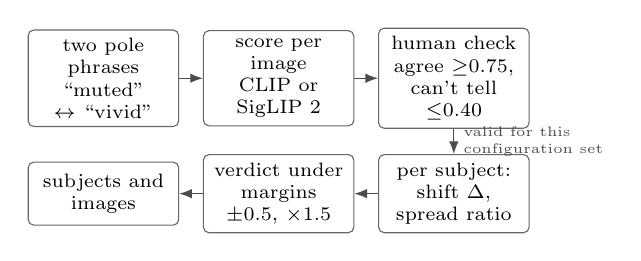
\begin{tikzpicture}[font=\scriptsize, node distance=3.2mm and 3mm,
  box/.style={draw=black!60, rounded corners=2pt, align=center, inner sep=3pt, minimum height=8mm, text width=17mm},
  arr/.style={-{Latex[length=1.6mm]}, black!70}]
\node[box] (poles) {two pole phrases\\``muted'' $\leftrightarrow$ ``vivid''};
\node[box, right=of poles] (score) {score per image\\CLIP or SigLIP~2};
\node[box, right=of score] (check) {human check\\agree $\geq$0.75,\\can't tell $\leq$0.40};
\node[box, below=of check] (eff) {per subject: shift $\Delta$,\\spread ratio};
\node[box, left=of eff] (verdict) {verdict under\\margins $\pm$0.5, $\times$1.5};
\node[box, left=of verdict] (imgs) {subjects and\\images};
\draw[arr] (poles) -- (score); \draw[arr] (score) -- (check); \draw[arr] (check) -- node[right, align=left, font=\tiny]{valid for this\\configuration set} (eff);
\draw[arr] (eff) -- (verdict); \draw[arr] (verdict) -- (imgs);
\end{tikzpicture}}
\caption{The measurement behind every view: an aspect is defined in words, scored by an encoder, checked by people for each configuration set, and turned into per-subject shift and spread with verdicts under explicit margins that lead back to the images.}
\label{fig:framework}
\end{figure}

\paragraph{Shift and spread.}
For a contrast A$\rightarrow$B, per subject and aspect, the shift is $\Delta = (\mathrm{median}_B - \mathrm{median}_A)/s$, where $s$ is a per-aspect scale frozen once from the 12 configurations (one unit is the typical spread of one configuration on one subject), and the spread ratio is $\mathrm{IQR}_B/\mathrm{IQR}_A$. Margins were frozen before any comparison was examined: a shift of at least 0.5 units is a displacement, a ratio beyond 1.5 or below 1/1.5 is a change in spread, and ``same place'' or ``same spread'' requires the 90\% interval to lie inside the margin. A hierarchical bootstrap resamples subjects within categories and images within cells, with seeds paired when A and B share a checkpoint. Primary tests are Holm-corrected; aspects, margins, scale and code, and for the LLM study also the rewriters, VLM prompts and scoring rules, were committed before each analysis. In the system, a change is marked only when the whole interval lies beyond the margin, which is stricter than the confirmatory rule (significant after correction, estimate beyond the margin).

\paragraph{Validity conditions.}
Every setting is declared; a contrast that changes several settings is a package and is not attributed to one of them; a pooled result is never read without its per-subject structure; baselines do not move when configurations are shown or hidden; measurement validity is stated per configuration set and encoder; and a claim stated in language is a hypothesis to check against the images.

\section{How Judging Without Visual Analysis Fails}
\label{sec:failures}

We report the experiments by the way of judging they test (\cref{fig:failures}).

\subsection{F1: Numbers without images mislead}

\paragraph{F1a: a number can measure the wrong thing.}
Three rounds of human checks decided which aspects enter the analysis (\cref{tab:validation}). In round~1 (240 pairs), 7 of 15 candidates passed and five were frozen: saturation, medium (photograph vs.\ painting), shot (close-up vs.\ wide), tone (modern vs.\ vintage) and background (plain vs.\ busy). ``Style'' ran backwards: CLIP called polished photographs ``stylized'', and people agreed with its direction on only 17\% of pairs. In round~2, validity did not transfer to the later, more homogeneous configurations. In round~3, on images from rewritten prompts, background agreement fell to 0.38: CLIP's ``busy'' was more often the opposite of people's reading than the same. The strongest result of the pre-registered rewriting study lies on exactly this axis: after rewriting, FLUX.2 dev's backgrounds move toward ``busy'' ($+0.67$ [$+0.47$, $+0.91$], 17 subjects up, none down). Read as a number, it would have been the headline finding.

\begin{table}[tb]
\caption{Agreement with the encoder on large-gap pairs, CLIP / SigLIP~2 ($\times$ = fails the frozen rule). Rounds: first six configurations, later six, images from rewritten prompts.}
\label{tab:validation}
\scriptsize\centering
\begin{tabular}{@{}lccc@{}}
\toprule
Aspect & Round 1 & Round 2 & Round 3 (rewrites) \\
\midrule
saturation & 0.92 / 0.92 & 0.77 / 0.73$\times$ & 0.90 / 0.90 \\
medium & 0.90 / 0.90 & 0.77 / 0.77 & 0.77 / 0.77 \\
shot & 0.90 / 0.90 & 0.96 / 0.96 & 0.63$\times$ / 0.75 \\
tone & 0.94 / 0.94 & 0.64$\times$ / 0.88 & 0.89 / 0.68$\times$ \\
background & 0.81 / 0.84 & 0.70$\times$ / 0.70$\times$ & 0.38$\times$ / 0.56$\times$ \\
\bottomrule
\end{tabular}
\end{table}

\paragraph{F1b: a pooled number hides opposite shifts.}
On validated aspects, 38 of the 60 pooled comparisons that fall within the margin hide opposite shifts, with at least three subjects beyond $+0.5$ and three beyond $-0.5$. SDXL$\rightarrow$SDXL-Turbo, a package of five settings, is the clearest case: every pooled shift is ``same place'' or unresolved, yet four of five aspects hide opposite shifts. On saturation, 9 subjects become more vivid and 6 more muted, each with its own interval excluding zero; ``a horse'' moves $+2.33$ while ``a bird on a branch'' moves $-2.07$ (\cref{fig:failures}a).

\paragraph{F1c: one number merges shift and narrowing, and the shift depends on the encoder.}
In klein-base 4B, raising guidance from 1 to 4 narrows four aspects beyond the margin (saturation $\times$0.51 [0.43, 0.61], medium $\times$0.53, tone $\times$0.49, background $\times$0.65) and shifts only saturation ($+0.65$ [$+0.43$, $+0.93$]); 15 of 24 subjects turn vivid by at least the margin and none muted. The distilled klein 4B (new checkpoint, 50$\rightarrow$4 steps) narrows all five aspects ($\times$0.41--0.63) and shifts saturation ($+0.95$): the guidance pattern, more strongly, as DefaultShift observed~\cite{defaultshift}. Under SigLIP~2 the narrowing holds (guidance $\times$0.52--0.62; distillation $\times$0.48--0.58, saturation $+1.03$), but guidance now shifts medium ($+1.08$), shot ($-0.86$) and tone ($-1.59$), and saturation falls below the margin ($+0.44$) (\cref{fig:failures}b). Per-subject readings agree only moderately between the encoders (median Spearman 0.33--0.67). A diversity score would report ``less diverse'' under both encoders and hide that only the narrowing is robust.

\begin{figure*}[tb]
\centering
\includegraphics[width=\linewidth]{fig3_failures.pdf}
\caption{Evidence for the three failure modes.
(a)~F1b: per-subject saturation shifts of SDXL$\rightarrow$SDXL-Turbo around a pooled shift of $+0.17$; coloured subjects lie beyond the margin (10 more vivid, 7 more muted; 9 and 6 of them also have an interval excluding zero).
(b)~F1c: klein-base 4B, guidance 1$\rightarrow$4, pooled shift and spread ratio with 90\% intervals under CLIP (filled) and SigLIP~2 (hollow); bands are the margins. The narrowing agrees; the shifts do not.
(c)~F2 and F3: on the same 48 grid pairs (8 vs.\ 8 images), both VLMs report a difference on every null pair, people on a third; people find 3 of 10 real shifts.}
\label{fig:failures}
\end{figure*}

\subsection{F2: Language without measurement asserts what is not there}
In the pre-registered VLM study, Qwen3.5-4B and Mistral-Small-3.2-24B saw 8 vs.\ 8 images per subject for six contrasts, as two grids, and gave a free-text description plus constrained answers per aspect (``closer to $\langle$right$\rangle$ / $\langle$left$\rangle$ / no clear difference''; ``more / less / about equally varied''), scored against the audit on all 32 seeds on validated aspects. After the first scoring we added, as exploratory checks, a null control (one configuration on both sides, seeds shifted by 16), a second disjoint draw of grids, and people answering the same questions (\cref{sec:f3}).

Both VLMs reported a shift between two sets from the same configuration in 98--100\% of answers (\cref{tab:vlm}). This is not sampling noise: a second draw gives the same answer in 88--93\% of cases, and where the eight shown seeds decide, they agree with the 32-seed truth in 98--100\% of cases. The VLMs also called narrowing movement (12--13 of 13 cases) and described a pooled shift in 49--50 of 50 pooled ``no change'' cases that hide reversals. Given a real difference, however, Mistral-24B reads the direction of variety correctly in 79\% of per-subject cases. Other language fails in the same way. Rewritten prompts move toward ``a photograph'' while their images move toward illustration ($+0.53$ and $+0.37$, not significant after correction), and per subject the text predicts the image only for saturation (Spearman 0.42--0.53). Six new axes proposed by a VLM (sharpness, level of detail, natural vs.\ idealized, contrast, lighting, texture) were understood by people (``can't tell'' in 11--25\% of judgements), but none passed the check (0.34--0.70).

\begin{table}[tb]
\caption{VLM answers against the audit; the lower block compares people and VLMs on the same 48 grid pairs.}
\label{tab:vlm}
\scriptsize\centering
\begin{tabularx}{\columnwidth}{@{}>{\raggedright\arraybackslash}Xccc@{}}
\toprule
 & Qwen-4B & Mistral-24B & People\textsuperscript{a} \\
\midrule
Per-subject shift accuracy & 0.49 & 0.48 & \\
Per-subject variety accuracy & 0.63 & 0.79 & \\
Narrowing without a shift, answered ``shift'' & 12/13 & 13/13 & \\
Hidden reversals described as a pooled shift & 49/50 & 50/50 & \\
\textbf{Null control: a shift reported} & \textbf{98\%} & \textbf{100\%} & \\
Same answer on a second draw & 0.88--0.91 & 0.88--0.93 & \\
\midrule
Null pairs reported as different & \textbf{12/12} & \textbf{12/12} & \textbf{4/12} \\
Real shifts, direction correct & 6/10 & 8/10 & 3/10 \\
Variety correct & 13/18 & 15/18 & 12/17 \\
\bottomrule
\multicolumn{4}{@{}l}{\textsuperscript{a}Majority of three annotators.}
\end{tabularx}
\end{table}

\subsection{F3: Eyes without measurement miss real differences}
\label{sec:f3}
Three annotators answered the VLMs' constrained questions on 48 of the same grid pairs (36 from the contrasts, 12 null pairs). On null pairs their majority reported a difference in 4 of 12, against 12 of 12 for both VLMs, so the VLMs' false alarms are not forced by the grids. On real shifts their majority found the direction in 3 of 10 (Mistral-24B: 8 of 10), and agreement among people was moderate (Fleiss' $\kappa$ 0.41 for shift, 0.54 for variety). Eight images per side are too few for a person to separate a default change from sampling noise, yet 32 images per side for 24 subjects and 12 configurations are more than anyone can read without guidance.

\subsection{What follows: tasks and requirements}
\label{sec:requirements}
No single way of judging is enough: numbers need the images and the per-subject structure, language needs a measurement to check it against, and eyes need the measurement to tell them where to look. An evaluator needs to move between all three, and visual analytics is how they can. From the failures and from the decisions evaluators take, we derive five tasks:
\begin{description}\itemsep0pt
\item[T1 Shift or narrowing:] does a change move the typical output, narrow it, or both, and under which encoder? (F1c)
\item[T2 Pooled or per subject:] does a pooled conclusion hold for every subject, and which subjects go against it? (F1b)
\item[T3 Trust a reading:] is the aspect valid for these configurations, and can the contrast be attributed to one setting? (F1a)
\item[T4 Verify a language claim:] is a VLM statement, a rewrite or an axis name supported by the images? (F2)
\item[T5 Compare many configurations:] along a chain or family, which members move or narrow appearance, and for which subjects?
\end{description}
and five requirements:
\begin{description}\itemsep0pt
\item[R1 Explore, do not report:] every verdict is computed from the data in view, under margins and an encoder the analyst can change. (F1c)
\item[R2 Many configurations, one reference:] configurations are compared as a set against an explicit reference, identified by position and label rather than hue. (T5)
\item[R3 Every reading reaches the images:] from any number, a path leads to its subjects and images, chosen by the measurement over all seeds. (F1b, F3)
\item[R4 Language is a hypothesis:] statements, rewrites and axis names are linked to the evidence that decides them; validity is shown per configuration and encoder; new axes count only after a human check. (F1a, F2)
\item[R5 Findings are reproducible:] a conclusion is stored with the full analysis state and can be replayed.
\end{description}
\Cref{tab:map} links each failure to its requirement, design, case and expert task.

\begin{table*}[tb]
\caption{From failure to design, case and evaluation.}
\label{tab:map}
\scriptsize\centering
\begin{tabularx}{\linewidth}{@{}>{\raggedright\arraybackslash}p{0.27\linewidth}c>{\raggedright\arraybackslash}Xcc@{}}
\toprule
Failure (evidence) & Requirement & Design in \sysname{} & Case & Expert task \\
\midrule
F1a an aspect measures the wrong thing (style; background on rewrites) & R4 & validity mark $\oslash$ per member and encoder; user-defined aspects with an in-tool check & \ref{sec:case63} & T3 \\
F1b pooled numbers hide reversals (38 of 60) & R3 & per-member shift columns, reversal badge, subject dots around the pooled diamond & \ref{sec:case62} & T2 \\
F1c shift and narrowing merged; shifts encoder-specific & R1 & shift $\times$ spread scatters, margin handles, encoder switch & \ref{sec:case61} & T1 \\
F2 VLMs assert differences; text and image disagree & R4, R3 & statements with live verdicts, audit trail, rewrite view & \ref{sec:case64} & T4 \\
F3 a few images are not enough & R3, R1 & images placed on the axis over all seeds, paired-seed lines, brushing & all & all \\
\bottomrule
\end{tabularx}
\end{table*}

\section{\sysname{}}
\label{sec:system}

\sysname{} is a single-screen web system built with D3, with five linked panels (\cref{fig:teaser}). It runs from disk; user-defined aspects need a local web server.

\subsection{The comparison set and the encoder (R1, R2)}
The header holds a comparison set of up to six configurations in chain order. The \emph{reference} (blue) is the configuration every contrast is measured from; the \emph{focus} (orange) is the member detailed by the per-subject views. Further members are drawn in ink and identified by their slot---a matrix column, an image lane, a parallel axis, a distribution row, a small multiple---and by a direct label, so hue never has to distinguish six members. A chip lists the declared settings that differ from the reference, and a warning chip appears when more than one differs, so the contrast is not attributed to one setting (T3). The \emph{encoder switch} (CLIP $|$ SigLIP~2) replaces the scores, the frozen scale and the validity of every aspect, and every view and verdict is recomputed; a finding that changes under the switch is encoder-specific (F1c).

\subsection{Panel A: where configurations settle}
The \emph{configuration map} (T1, T5) places each configuration at its typical location (x) and spread (y) on the chosen aspect; families are shapes, and arrows join designed contrasts (solid: guidance only; dashed: a package; dotted: prompt rewriting). Density contours of the 24 per-subject positions show whether a member behaves consistently across subjects, and semantic zoom keeps the estimate fixed in scale units. The \emph{contrast overview} gives one row per contrast and one glyph per aspect: an arrow for the pooled shift (dashed while its interval reaches into the margin), a disc against a unit ring for the spread ratio, and a count of subjects against the pooled direction. The \emph{statement view} (T4) places each VLM statement about the pair as a glyph in a subject $\times$ aspect grid; colour and a symbol give the audit's verdict (confirmed, narrowed but did not move, no shift, contradicted), recomputed live from the current data, margins and encoder (R1), with the frozen verdict shown when the two differ. The \emph{audit trail} (T3, T4) follows one claim---a statement, a rewrite or an axis name---through the measurement that decides it and one subject to its images (same seed, or rank-matched and labelled so), with a verdict on each link.

\subsection{Panels B--E: from subjects to images (R3)}
Panel~B (T2) colours each subject $\times$ configuration cell by where the configuration puts the subject between the poles; one shift column per member shows each subject's shift from the reference on a common scale, subjects that move against that member's pooled direction beyond the margin are outlined, and a badge steps through them. Panel~C (T3) places every image of the selected subject by its score, one lane per member, with the margin band and each member's median: the measurement over all seeds decides where to look, and the images show what the number means (F3). Panel~D (T1, T5) shows the same seeds as parallel coordinates through all members---joined seed by seed where members share the starting noise, rank-matched and dashed otherwise, so that leaning lines read as a shift and converging lines as a narrowing---and alternatively the subject's distributions on every aspect, an appearance map (a shared t-SNE of image embeddings, one small multiple per member) and, for rewriting contrasts, each rewrite placed by what its text says against where its image lands. Panel~E (T1, T2) has one scatter per aspect, each subject a dot at (shift, log spread ratio) with its interval, the margins as bands, and the pooled estimate and further members as labelled diamonds. Dragging the margin handles changes the margins for exploration and every verdict updates; brushing subjects highlights them everywhere and adds their median for every member; an aspect not validated for a member under the current encoder is marked $\oslash$.

\subsection{User-defined aspects with an in-tool check (R4)}
An analyst types two pole phrases. The phrases are embedded in the browser with the same CLIP text encoder, bundled and run locally (the ONNX export matches PyTorch at cosine 1.0000), and every image is scored from its stored embedding exactly as the frozen aspects; on first use, the tool reproduces the stored saturation scores of all 12,288 images within 0.004 scale units. The new aspect enters every view at once, marked $\oslash$. The analyst then judges 12 large-gap pairs from the current set, blind to configuration and score and sampled as in round~1 (one image from a subject's top 15\%, one from its bottom 15\%), and the frozen rule decides whether the aspect counts for these configurations. The result is stored with the aspect and in the findings log. This turns F1a and the failed VLM-proposed axes into an interaction: words do not measure images until a person confirms they do.

\subsection{Provenance and design rationale}
Choosing a member, aspect or subject in any view updates every other view. A finding recorded from any view is stored with the whole analysis state---set and roles, encoder, aspect, subject, panel modes, margins, brushed subjects, statement, map zoom---and replays on a click (R5). Each quantity has one home view (effects in E, images in C, distributions in D), and overviews restate a number only as a pointer to its home; density contours appear only on metric spaces; no status relies on colour alone. We discarded convex hulls on the projection, which readers took for spread; baselines that changed with the visible configurations; and summary cards that pooled all prompts and hid exactly the reversals of T2.

\section{Cases}
\label{sec:cases}
Each case starts from a failure of \cref{sec:failures} and follows an analyst through \sysname{} on the real data. The findings were first established by the scripted analyses; the cases show how the system reaches and checks them, and what it adds that a number, a sentence or a few images do not.

\subsection{Shift, narrowing, or the encoder? (F1c; T1, T5)}
\label{sec:case61}
With klein-base 4B at guidance 1 as reference, guidance 4 as focus and the distilled klein 4B as a third member (\cref{fig:case61}), panel~E shows the focus's diamonds below the spread band on four aspects and the distilled member's further down on all five; only saturation's lies right of the shift band. In panel~D the seed lines lean right and converge from guidance 1 to 4; the segment to klein 4B is rank-matched and dashed, because its checkpoint differs. Switching to SigLIP~2 keeps the diamonds below the spread band, but on medium the focus now moves toward illustration ($+1.08$) and the map shows its arrow leaving the reference. Dragging the spread margin shows how robust the narrowing is: medium, tone and saturation stay narrowed, with their whole interval beyond the margin, up to a margin of $\times$1.52--1.62, background and shot only up to $\times$1.26 and $\times$1.20. The analyst logs ``narrows like guidance, more strongly; which aspects move is encoder-specific'' with both states. Without the system, a diversity score says ``less diverse'' under both encoders, and a single-encoder analysis reports its own shifts as facts.

\begin{figure*}[tb]
\centering
\includegraphics[width=\linewidth]{fig5_case61.png}
\caption{Case \ref{sec:case61}: the same view of klein-base 4B, guidance 1$\rightarrow$4$\rightarrow$distilled, on medium under CLIP (left) and SigLIP~2 (right): configuration maps, then the medium and tone scatters. Under both encoders the diamonds lie below the spread band (narrowing); only under SigLIP~2 does guidance move medium toward illustration.}
\label{fig:case61}
\end{figure*}

\subsection{A pooled ``no change'' that hides reversals (F1b; T2, T3)}
\label{sec:case62}
The contrast overview shows SDXL$\rightarrow$SDXL-Turbo with short arrows and a large reversal count. With the pair as reference and focus, the pooled saturation diamond sits inside the shift band with subject dots on both sides (\cref{fig:cases6263}a). The badge (7) steps through the subjects that turn muted beyond the margin against the slightly positive pooled shift---``a bird on a branch'', ``a car'', ``a kitchen'', ``a library'', ``a city street'', ``a mountain'', ``a picnic''---while in the shift column ``a horse'' and ``a cup of coffee'' are the longest bars on the vivid side. In panel~C, Turbo's images of the horse sit on the vivid side and those of the bird on the muted side. The warning chip lists five differing settings, so the finding is not attributed to distillation. Without the system, the pooled number says ``no difference'', and eight images of one subject show only one direction.

\begin{figure*}[tb]
\centering
\includegraphics[width=\linewidth]{fig6_cases_62_63.png}
\caption{(a)~Case \ref{sec:case62}: SDXL$\rightarrow$SDXL-Turbo on saturation; subjects lie on both sides of a pooled diamond inside the margin, and the image lanes show one subject each way. (b)~Case \ref{sec:case63}: FLUX.2 dev with and without its official rewriter; the strongest effect (background, toward busy) lies on an aspect not validated for rewritten images ($\oslash$), and the picnic images scored ``busy'' look like the originals; medium's ratio stays inside the spread band.}
\label{fig:cases6263}
\end{figure*}

\subsection{Auditing a prompt rewriter (F1a, F2; T3, T4)}
\label{sec:case63}
Comparing FLUX.2 dev with its rewritten-prompt version, panel~E shows the strongest effect, toward a busy background, but the card carries $\oslash$ (\cref{fig:cases6263}b). In panel~C, for ``a picnic'', the subject with the largest shift, the rewritten images are scored far toward ``busy'', yet they show the same kind of grassy scene as the originals---the failure the round-3 check measured. On validated aspects the diamonds of saturation ($\times$1.31) and medium ($\times$1.49) stay inside the spread band; medium's interval reaches beyond it, so widening is undecided, not shown. In the rewrite view, rewrites whose text leans toward ``photograph'' sit next to images that drifted toward illustration. Without the system, the strongest number would have become the headline, and the rewriter's text would have suggested the opposite of what the images show.

\subsection{Checking what a VLM says (F2, F3; T4)}
\label{sec:case64}
In the statement view for SDXL$\rightarrow$Turbo, a Mistral-24B statement about ``a restaurant'' reads: ``Set B images include more detailed architectural elements such as arched windows and ornate moldings.'' It is coded to background, toward busy, and marked contradicted; Qwen3.5-4B made nearly the same claim, which the coder placed outside the measured aspects. The audit trail (\cref{fig:case64}) shows the restaurant's backgrounds becoming much plainer ($-1.68$ [$-2.95$, $-1.15$]) and less varied ($\times$0.12) while the pooled shift is $+0.11$, so the trail also marks that pooling hides the subject; the images confirm it. A statement about ``a car''---``Set B images have a more sepia tone and muted color palette''---is confirmed by tone moving toward vintage ($+1.44$) and saturation toward muted ($-1.47$). Of the 290 statements about this pair, 94 fall outside or beside the measured aspects, 74 cannot be decided by the audit, 112 are confirmed (most about variety), 6 claim a shift the audit does not find and 4 are contradicted; for klein guidance, 11 statements describe a narrowing as a change in look. Dragging the shift margin or switching the encoder changes some verdicts live, which shows which statements are robust. Without the system the sentence reads as plausible, and eight images per side do not settle it either, because people miss most real shifts there (F3).

\begin{figure}[tb]
\centering
\includegraphics[width=\columnwidth]{fig7_case64.png}
\caption{Case \ref{sec:case64}: a VLM statement about SDXL$\rightarrow$Turbo traced through the measurement (pooled $+0.11$, the restaurant $-1.68$) and the subject to its images, with a verdict on each link.}
\label{fig:case64}
\end{figure}

\subsection{Defining and checking a new aspect (F1a; R4)}
\pending{To be run on the real data: the analyst suspects that guidance and distillation push scenes toward daylight, defines ``a scene in daylight'' $\leftrightarrow$ ``a scene at night'', inspects it in every view and checks it on the set; for contrast, the VLM-proposed pair that failed round~3 (``rich detail'' $\leftrightarrow$ ``minimal detail'', 0.34) is entered and checked.}

\section{Expert Study}
\label{sec:study}
\pending{Pending. The design is fixed; results follow the sessions.}
The study asks whether the visual analysis helps experts avoid the failures of \cref{sec:failures}, compared with the same numbers and images without it. Five researchers who train, evaluate or select generative image models (5--10 years in imaging research), at least two from outside the authors' group, solve T1--T4 twice, once with \sysname{} and once with a baseline, on different cases of the same kind; condition order and case assignment are counterbalanced, and a pilot session precedes them. The baseline has the same pooled and per-subject numbers with intervals, the settings, the validation table, sortable image grids and the VLM statements as text, but no visual encoding of effects and no linking. Each task targets one failure: T1 (F1c), T2 (F1b), T3 (F1a), T4 (F2). We record correctness by rules fixed in advance, scored by a second judge blind to condition, the evidence cited, confidence and time, and we hold an interview. Results are reported descriptively. Because the tool displays the audit, correctness with the tool partly means reading the audit correctly; the baseline shows the same numbers, so the comparison isolates visual encoding and linking.

\section{Discussion}

\paragraph{Why visual analysis, and not a better score or a better VLM.}
The three ways of judging failed in complementary ways. Numbers were wrong when the measure was wrong, pooled or encoder-specific; language asserted differences that were not there; eyes on a few images missed real differences. Each failure is repaired by what another way provides: numbers by a look at the images, language by a measurement, and eyes by a measurement over all seeds that tells them where to look. A visual analytics system is where these meet. This is the sense in which the visualization is necessary here: it is not an illustration of results computed elsewhere, but the place where measurement, language and human judgement check one another.

\paragraph{Language proposes, images decide.}
The results suggest a division of labour for LLM-assisted visual analytics: language models propose candidates, suspected differences and summaries, and a visual analysis with validated measures, explicit margins and a path to the images decides. \sysname{} builds this into the interface: statements are hypotheses with verdicts, and new axes must pass a check before they count.

\paragraph{Generality.}
The design needs configurations rendered on shared prompts and seeds, a measurement that can be defined in words, a human check for it, and per-unit effects with uncertainty. These carry over to video or text-to-3D defaults and to comparing LLM outputs along language-defined attributes.

\paragraph{Limitations.}
CLIP and SigLIP aspects are approximations, and shift findings are encoder-specific; validity under SigLIP is judged on pairs sampled by CLIP gaps, which favours CLIP. The 0.5 margin is not a perceptual unit, and native resolutions differ (512--1328\,px). The language data use one rewriter instruction and two open VLMs with one prompt format, and the human grid check has three annotators and 48 items. The comparison set holds six members, and the expert study is small and formative.

\section{Conclusion}
Evaluators judge how text-to-image defaults change by numbers, by language, or by looking at a few images. On 12 open configurations each of these failed on its own: numbers measured the wrong thing, hid reversals and depended on the encoder; VLMs reported differences that were not there; people with eight images missed real differences. \sysname{} combines the three: it computes verdicts over all seeds under margins and encoders the analyst can change, leads every number and claim to its images, and lets the analyst define and check new aspects.

\section*{Supplemental Materials}
\pending{Anonymized link for review.} The supplemental materials contain the pre-registrations, analysis code and result tables, the human validation protocols and aggregated answers, the audit tool with its data (runs offline), and a video of the cases.

\section*{AI Use Disclosure}
\pending{To be confirmed by the authors.} An AI assistant (Claude, Anthropic) was used to write analysis and system code, to draft and edit the text, and to produce figures from the authors' data and system; the authors designed the study, checked every result against the data, and take responsibility for the content.

\acknowledgments{\pending{Annotators; experts; funding.}}

\bibliographystyle{abbrv-doi}
\bibliography{refs}
\end{document}
